\documentclass[11pt]{ctexart}

\usepackage{geometry}
\geometry{
    left = 0.6in,
    right = 0.6in,
    top = 0.8in,
    bottom = 1.0in
}
\usepackage{amssymb,amsbsy,amsmath,xcolor,mathrsfs,graphicx}
\usepackage{listings}
\usepackage{tasks}
\usepackage{pifont}
\settasks{
    label = \Alph*. ,
    label-width = 16pt
}

\renewcommand{\title}[3]{
    \begin{center}
        \Large\heiti 中国电子学会 #1~年~#2~月 Python~#3级考试
    \end{center}
}
\newcommand{\TimeAndName}[1]{
    \begin{center}
        考试时间:~#1~ 分钟 \qquad\qquad\qquad\qquad 姓名:\underline{\quad\quad\quad\quad}
    \end{center}
}

\begin{document}
    \lstset{
        language = python,
        keywordstyle = \color{orange}\bfseries,
        emph = {
            abs, all, any, ascii, bin, bool, breakpoint, bytearray, bytes,
            callable, chr, classmethod, compile, complex, copyright, credits,
            delattr, dict, dir, divmod, enumerate, eval, exec, exit, filter,
            float, format, frozenset, getattr, globals, hasattr, hash,
            help, hex, id, input, int, isinstance, issubclass, iter, len,
            license, list, locals, map, max, memoryview, min, next, object,
            oct, open, ord, pow, print, property, quit, range, repr, reversed,
            round, set, setattr, slice, sorted, staticmethod, str, sum, super,
            tuple, type, vars, zip,
        },
        emphstyle = \color{purple}\bfseries,
        showspaces = false,
        basicstyle = \ttfamily,
        morekeywords = {True,False}
    }

    \title{2022}{6}{一}
    
    \TimeAndName{60}
    
    {\noindent\heiti 第一部分、单选题(共 25 题,每题 2 分,共50分.)}

    \begin{enumerate}
        % 1
        \item 已知 \lstinline{a="161"}, \lstinline{b="16"}, \lstinline{c="8"},执行下列语句,变量\lstinline{d} 的值为多少?(\qquad)
        \begin{lstlisting}
            d = a > b and a > c
        \end{lstlisting}
        \begin{tasks}(4)
            \task 0
            \task 1
            \task \lstinline{True}
            \task \lstinline{False}
        \end{tasks}
    
        % 2
        \item 执行下列语句,变量 \lstinline{flag} 的值是多少?(\qquad)
        \begin{lstlisting}
            flag = "3456" > "36"
        \end{lstlisting}
        \begin{tasks}(4)
            \task \lstinline{"3456"}
            \task \lstinline{"36"}
            \task \lstinline{True}
            \task \lstinline{False}
        \end{tasks}

        % 3
        \item 执行语句 \lstinline{y = 123 % 100} 后,变量 \lstinline{y} 的值为?(\qquad)
        \begin{tasks}(4)
            \task 1
            \task 3
            \task 12
            \task 23
        \end{tasks}
    
        % 4
        \item Python 是一种(\qquad)编程语言?
        \begin{tasks}(4)
            \task 低级
            \task 高级
            \task 机器
            \task 汇编
        \end{tasks}

        % 5
        \item 以下哪种输入不可以得到以下反馈:\textbf{重要的事情说三遍:戴口罩!戴口罩!戴口罩!}?(\qquad)
        \begin{tasks}
            \task \lstinline{print("重要的事情说三遍:戴口罩!戴口罩!戴口罩!")}
            \task \lstinline{print("重要的事情说三遍:" + "戴口罩!" * 3)}
            \task \lstinline{print('重要的事情说三遍:' + '戴口罩!' * 3)}
            \task \lstinline{print("重要的事情说三遍:戴口罩!" * 3)}
        \end{tasks}

        % 6
        \item 在 Python 函数中,用户获取用户输入的是?(\qquad)
        \begin{tasks}(4)
            \task \lstinline{str()}
            \task \lstinline{eval()}
            \task \lstinline{print()}
            \task \lstinline{input()}
        \end{tasks}

        % 7
        \item 关于 Python 赋值语句,以下选项中不合法的是?(\qquad)
        \begin{tasks}(4)
            \task \lstinline{a, b = b, a}
            \task \lstinline{a = b = 1}
            \task \lstinline{a = (b = 1)}
            \task \lstinline{a = 1; b = 1}
        \end{tasks}

        % 8
        \item 在 Python 中输入 \lstinline{2 + 7 / 2},输出结果为哪一种数据类型?(\qquad)
        \begin{tasks}(4)
            \task 整数型
            \task 浮点型
            \task 字符型
            \task 文字型
        \end{tasks}

        % 9
        \item 在 Python g中,\lstinline{a = 2, b = "3.5"},如果想进行 \lstinline{ 2 + 3.5} 的加法运算,我们应该如何编写代码?(\qquad)
        \begin{tasks}(4)
            \task \lstinline{a + b}
            \task \lstinline{str(a) + b}
            \task \lstinline{a + int(b)}
            \task \lstinline{a + eval(b)}
        \end{tasks}

        % 10
        \item 算术运算符、比较运算符和逻辑运算符,在 Python 中的运算中的优先关系是?(\qquad)
        \begin{tasks}(2)
            \task 算术运算符 > 比较运算符 > 逻辑运算符
            \task 比较运算符 > 逻辑运算符 > 算术运算符
            \task 算术运算符 > 逻辑运算符 > 比较运算符
            \task 逻辑运算符 > 比较运算符 > 算术运算符
        \end{tasks}

        % 11
        \item 图形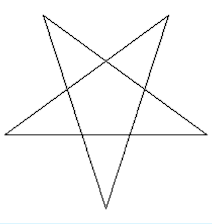
\includegraphics[width=.05\textwidth]{11.png}最有可能是哪个选项的代码执行后的效果?(\qquad)
        \begin{tasks}(2)
            \task \lstinline{import turtle as t}\\
            \lstinline{t.forward(200)}\\
            \lstinline{t.right(144)}\\
            \lstinline{t.forward(200)}\\
            \lstinline{t.left(144)}\\
            \lstinline{t.forward(200)}\\
            \lstinline{t.left(144)}\\
            \lstinline{t.forward(200)}\\
            \lstinline{t.right(144)}\\
            \lstinline{t.forward(200)}\\
            \lstinline{t.hideturtle()}

            \task \lstinline{import turtle as t}\\
            \lstinline{t.forward(200)}\\
            \lstinline{t.left(144)}\\
            \lstinline{t.forward(200)}\\
            \lstinline{t.left(144)}\\
            \lstinline{t.forward(200)}\\
            \lstinline{t.left(144)}\\
            \lstinline{t.forward(200)}\\
            \lstinline{t.left(144)}\\
            \lstinline{t.forward(200)}\\
            \lstinline{t.hideturtle()}

            \task \lstinline{import turtle as t}\\
            \lstinline{t.forward(200)}\\
            \lstinline{t.right(144)}\\
            \lstinline{t.backward(200)}\\
            \lstinline{t.left(144)}\\
            \lstinline{t.forward(200)}\\
            \lstinline{t.left(144)}\\
            \lstinline{t.backward(200)}\\
            \lstinline{t.right(144)}\\
            \lstinline{t.forward(200)}\\
            \lstinline{t.hideturtle()}

            \task \lstinline{import turtle as t}\\
            \lstinline{t.forward(200)}\\
            \lstinline{t.left(144)}\\
            \lstinline{t.backward(200)}\\
            \lstinline{t.left(144)}\\
            \lstinline{t.forward(200)}\\
            \lstinline{t.left(144)}\\
            \lstinline{t.backward(200)}\\
            \lstinline{t.left(144)}\\
            \lstinline{t.forward(200)}\\
            \lstinline{t.hideturtle()} 
        \end{tasks}

        % 12
        \item \lstinline{print(1024//10**2)} 的结果是?(\qquad)
        \begin{tasks}(4)
            \task 100
            \task 24
            \task 10
            \task 10.24
        \end{tasks}

        \newpage
        % 13
        \item  \lstinline{turtle.reset()} 命令的含义是下列哪一种?(\qquad)
        \begin{tasks}
            \task 不清空 \lstinline{turtle} 窗口,重置 \lstinline{turtle} 的位置和状态
            \task 清空 \lstinline{turtle} 窗口,重置 \lstinline{turtle} 为初始状态
            \task 清空 \lstinline{turtle} 窗口,但是 \lstinline{turtle} 的位置和状态不会改变
            \task 撤销上一个动作
        \end{tasks}

        % 14
        \item \lstinline{turtle} 中画笔粗细为 5,我们调用 \lstinline{turtle.dot(None, "red")} 函数画点时,点的直径是多少(\qquad)?
        \begin{tasks}(4)
            \task 5
            \task 10
            \task 18
            \task 20
        \end{tasks}
        
        % 15
        \item 函数 \lstinline{turtle.circle(50, step=4)},画的是什么图形(\qquad)?
        \begin{tasks}(2)
            \task 直径是 50 的圆
            \task 对角线为 50 的正方形
            \task 对角线为 100 的正方形
            \task 边长是 50 的正方形
        \end{tasks}

        % 16
        \item 使用下面选项中的代码组合成一个 \lstinline{turtle} 文件中的一部分,来绘制一个空心五角星的脚本中,最不可能用到下面哪条代码(\qquad)?
        \begin{tasks}(4)
            \task \lstinline{t.left(144)}
            \task \lstinline{import turtle}
            \task \lstinline{t.circle(36)}
            \task \lstinline{t=turtle.Pen()}
        \end{tasks}

        % 17
        \item 以下不属于 Python 常见编程环境的是(\qquad)?
        \begin{tasks}(2)
            \task \lstinline{IDLE}
            \task \lstinline{Visual studio code}
            \task \lstinline{Java}
            \task \lstinline{Jupyter Notebook}
        \end{tasks}

        % 18
        \item 在 \lstinline{turtle} 库中的指令,执行以下代码指令后,画笔为哪种颜色(\qquad)?
        \begin{lstlisting}
            import turtle
            turtle.pencolor("yellow")
            turtle.color("green")
        \end{lstlisting}
        \begin{tasks}(4)
            \task 粉色
            \task 黄色
            \task 绿色
            \task 程序报错
        \end{tasks}

        % 19
        \item 假设 \lstinline{x = 14, y = 6},那么执行 \lstinline{x > y and 5},的结果为?(\qquad)
        \begin{tasks}(4)
            \task \lstinline{x > y}
            \task \lstinline{5}
            \task \lstinline{False}
            \task \lstinline{True}
        \end{tasks}

        % 20
        \item 以下哪个变量名是符合 Python 变量命名规范的(\qquad)?
        \begin{tasks}(4)
            \task 123
            \task \lstinline{my car}
            \task \lstinline{my_variable}
            \task \lstinline{&var}
        \end{tasks}

        % 21
        \item 已知:\lstinline{a = 7, b = 5, c = 12} 执行以下哪个语句结果为 \lstinline{True}?(\qquad)
        \begin{tasks}(4)
            \task \lstinline{a > c or a < b}
            \task \lstinline{a < c}
            \task \lstinline{a < c and a < b}
            \task \lstinline{c < b}
        \end{tasks}

        \newpage
        % 22
        \item 执行 \lstinline{7 * 8 - 6 > 10} 输出的结果是?(\qquad)
        \begin{tasks}(4)
            \task 56
            \task 50
            \task \lstinline{False}
            \task \lstinline{True}
        \end{tasks}

        % 23
        \item 关于 Python 以下说法正确的是?(\qquad)
        \begin{tasks}
            \task Python 安装好后,IDLE 也需要提前安装才可以用
            \task windows 自带的有 Python 环境,不需要安装
            \task 在 IDLE shell 的界面里显示有 Python 的版本
            \task 从 IDLE 新建文件,里面默认不是空的
        \end{tasks}

        % 24
        \item 关于 \lstinline{turtle} 库的引入,以下哪个是错误的?(\qquad)
        \begin{tasks}(2)
            \task \lstinline{import turtle}
            \task \lstinline{from turtle import *}
            \task \lstinline{import turtle as t}
            \task \lstinline{import turtle from t}
        \end{tasks}

        % 25
        \item 以下关于逻辑运算说法正确的是?(\qquad)
        \begin{tasks}
            \task 若 \lstinline{a = 10, b = 20, a and b} 的结果 10
            \task 若 \lstinline{a = 10, b = 20, a or b} 的结果是 20
            \task 若 \lstinline{a = 10, b = 20, not(a and b)} 的结果是 \lstinline{False}
            \task 若 \lstinline{a = 10, b = 20, not(a or b)} 的结果是 \lstinline{True}
        \end{tasks}
    \end{enumerate}

    {\noindent\heiti 第二部分、判断题(共 10 题,每题 2 分,共20分.)}
    \begin{enumerate}
        \setcounter{enumi}{25}
        % 26
        \item Windows 安装了 Python 环境下,在 CMD 命令行中,可以使用 \lstinline{C:\> python3 test.py} 执行 Python 文件 \lstinline{test.py} 中的指令(\qquad)

        %27
        \item 在 IDLE 编辑器中,Python 代码只能以一种颜色显示代码内容(\qquad)
        
        %28
        \item \lstinline{print(2 + eval("3"))} 运行结果为 5(\qquad)
  
        %29
        \item 在 Python 中变量需要提前定义,否则运行程序的时候不识别(\qquad)
        
        %30
        \item \lstinline{turtle.setup(width=0.5, height=0.75, stratx=None, starty=None)}设置画布的大小和位置(\qquad)
        
        %31
        \item Python 中的注释符号可分为单行注释和多行注释,单行注释符号是 \#(\qquad)
        
        %32
        \item \lstinline{type()} 函数用于返回对象的类型,那 \lstinline{print(type("3"))},输出结果为 \lstinline{<class 'int'>} (\qquad) 
        
        %33
        \item 语句1:\lstinline{print("Hello", end="")},\lstinline{print("World")};语句2:\lstinline{print("Hello")},\lstinline{print("World")};语句 1 和语句 2 的输出结果一样(\qquad)
        
        %34
        \item 可以将 \lstinline{a = "3.14"} 转化为浮点数的函数是 \lstinline{str()}(\qquad)
        
        %35
        \item \lstinline{turtle} 是 Python 内置的标准库,直接使用 \lstinline{import turtle} 导入使用即可,不用额外安装(\qquad)
    \end{enumerate}

    \newpage
    {\noindent\heiti 第三部分、编程题(共 2 题,共30分.)}
    \begin{enumerate}
        \setcounter{enumi}{35}
        
        % 36
        \item 买本子:小明同学带了一些前去帮同学买本子。请根据所带的元、单价和数量,算一算前够不够。
        
        \begin{tasks}[label=(\arabic*)]
            \task 程序运行后,输入三次数字(不能一次输完),这三个数字为整数,表示所带的元、单价和数量;
            \task 输出一行,钱足够买就输出 \lstinline{True},钱不够买就输出 \lstinline{False}
        \end{tasks}

        【输入样例】:

        100

        9

        11

        【输出样例】:
       
        \lstinline{True}
        \vfill

        %37
        \item 请使用 \lstinline{turtle} 画出如下标志:
        
        \begin{minipage}{.55\textwidth}
            \begin{tasks}[label=(\arabic*)]
                \task 线条颜色为黑色,线条粗细为 10;
                \task 圆半径为 50,填充颜色为蓝色;
                \task 等边三角形边长为 180;
                \task 等边三角形底边中点为画布正中心
            \end{tasks}
        \end{minipage}
        \begin{minipage}{.35\textwidth}
            \centering
            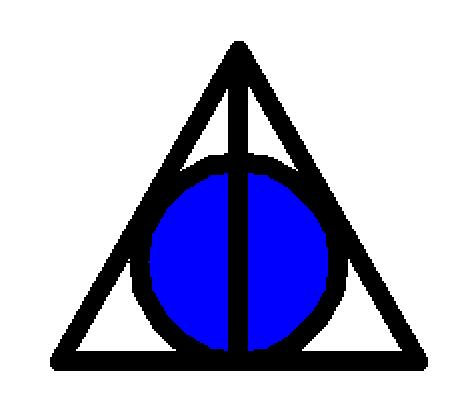
\includegraphics[width=0.5\textwidth]{37.jpg}
        \end{minipage}
        \vfill
    \end{enumerate}
\end{document}